\documentclass[xcolor=svgnames,17pt]{beamer}

\usepackage[export]{adjustbox}
\usepackage{bookmark}
\usepackage{colortbl} \arrayrulecolor[gray]{0.7}
\usepackage{microtype}
\usepackage{pgfpages}
\usepackage{rotating}
\usepackage{textcomp}
\usepackage{tabularx}
\usepackage{xspace}

\usepackage{fontspec}

\hypersetup{hidelinks,pdfpagemode=}

\urlstyle{same}

\newcommand*{\sizefont}[1]{%
    \ifcase#1\relax
    \or \tiny
    \or \scriptsize
    \or \footnotesize
    \or \small
    \or \normalsize
    \or \large
    \or \Large
    \or \LARGE
    \or \huge
    \or \Huge
    \fi}

%%

\newcommand*{\mybullet}{\tikz[baseline=-.6ex]\node[%
    draw,circle,inner sep = -0.15ex,fill]{.};\xspace}

\setbeamertemplate{footline}{
    \usebeamercolor[fg]{page number in head/foot}%
    \usebeamerfont{page number in head/foot}%
    \hfill\hspace*{1ex}\insertframenumber\,/\,\inserttotalframenumber\ 
    }

\newcommand*{\plainfooter}{%
    \setbeamertemplate{footline}{
        \usebeamercolor[fg]{page number in head/foot}%
        \usebeamerfont{page number in head/foot}%
        \hspace*{1ex}\insertframenumber\,/\,\inserttotalframenumber\vskip2pt}}

\makeatletter
\def\alphslide{\@alph{\intcalcAdd{1}{\intcalcSub{\thepage}{\beamer@framestartpage}}}}
\newcommand*{\plainstepfooter}{
    \setbeamertemplate{footline}{
        \usebeamercolor[fg]{page number in head/foot}%
        \usebeamerfont{page number in head/foot}%
        \hspace*{1ex}\insertframenumber\alphslide\,/\,\inserttotalframenumber\vskip2pt}}
\makeatother

\setbeamertemplate{note page}{
    \sizefont{3}
    \setlength{\parskip}{10pt}
    \insertnote
    \par}

\setbeamertemplate{navigation symbols}{}
\setbeamerfont{title}{size=\LARGE}
\setbeamerfont{frametitle}{size=\LARGE}
\setbeamerfont{framesubtitle}{size=\normalsize}

\newcommand*{\tocsection}[1]{\pdfbookmark[2]{#1}{#1}}

%%

\title{Modern Websites with Django and React}

\author{\texorpdfstring{%
    Andrew Neitsch}{Andrew Neitsch}}

\date{\small 2016-08-23}

\begin{document}

\tocsection{Title page}

\section{Introduction}

\begin{frame}[plain]
\titlepage
\end{frame}

\begin{frame}{}
\tableofcontents
\end{frame}

\begin{frame}{Disclaimer}

\begin{itemize}
\item I don’t know a lot about this
\pause
\item Was starting a new project, looked into what’s new in web development
\pause
\item Worked on this presentation instead of the project, so just a
beginner right now
\end{itemize}

\pause

\alert{If you know a better way to do this, please give a talk on it}

\end{frame}

\section{1. Django tutorial}

\begin{frame}{}
\tableofcontents[currentsection]
\end{frame}

\begin{frame}[fragile]{Django tutorial}

\sizefont{3}
\href{https://docs.djangoproject.com/en/1.10/intro/tutorial01/}{%
    \structure{https://docs.djangoproject.com/en/1.10/intro/tutorial01/}}

\end{frame}

\begingroup
\setbeamercolor{background canvas}{bg=gray}

\begin{frame}[plain]
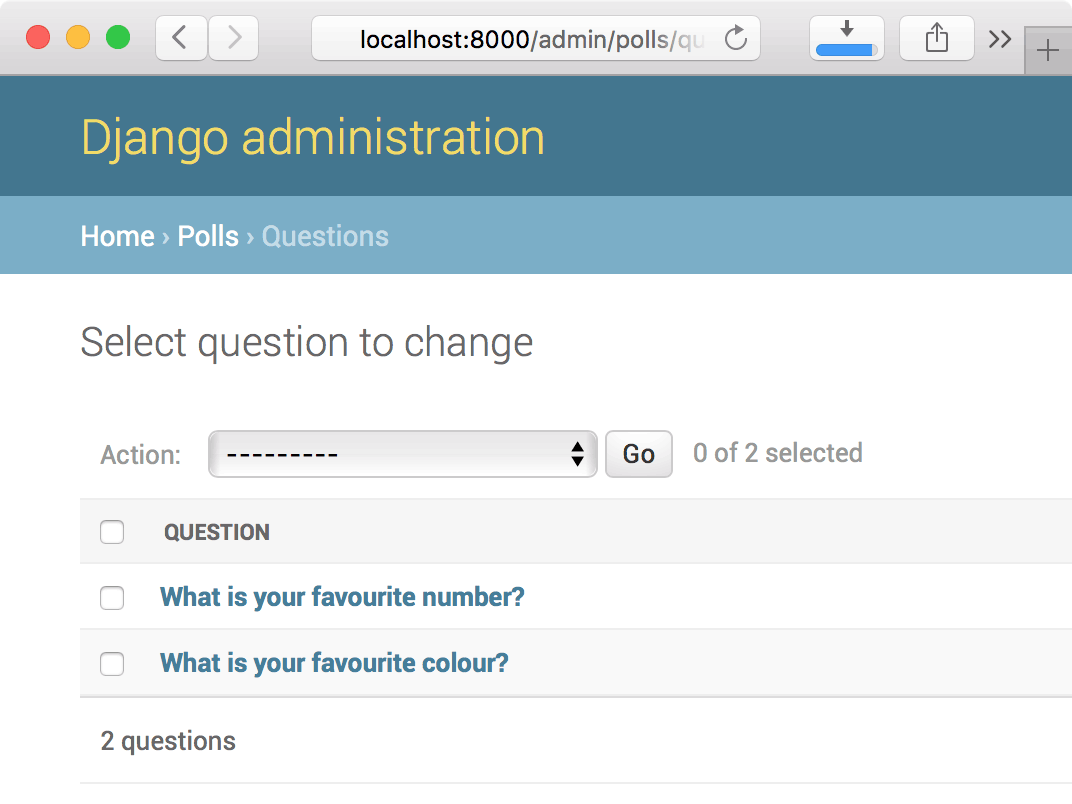
\includegraphics[width=0.95\paperwidth,center]{polls1.png}
\end{frame}

\begin{frame}[plain]
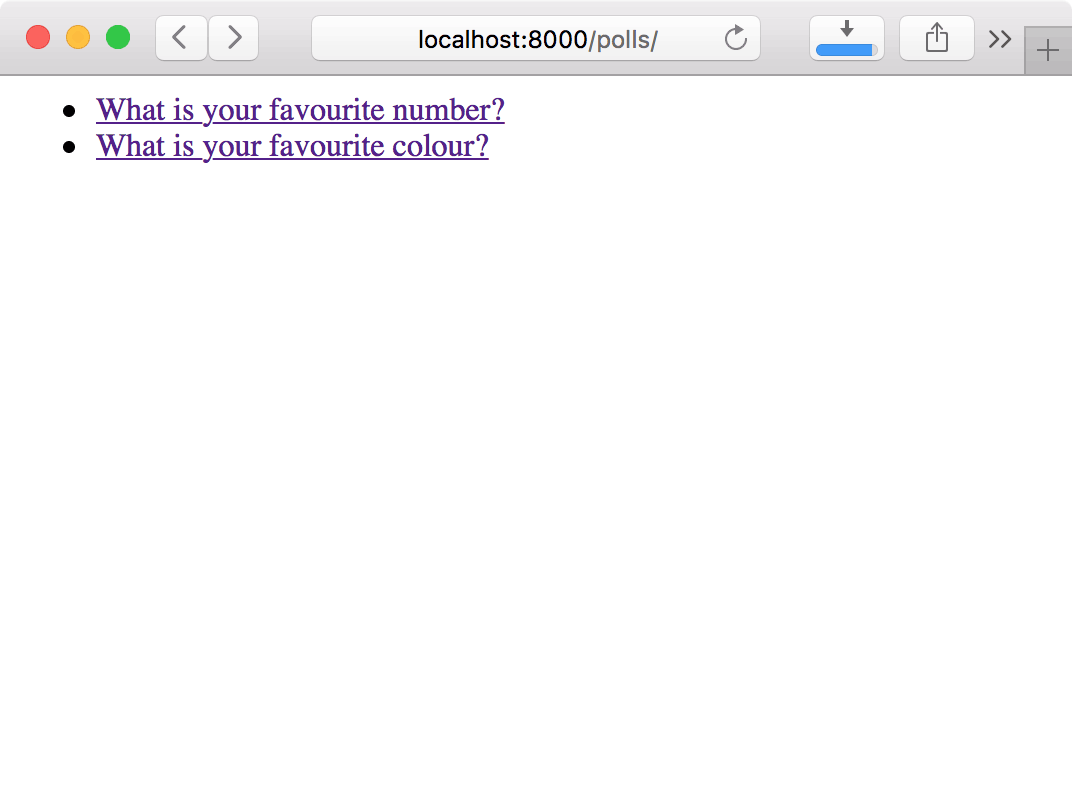
\includegraphics[width=0.95\paperwidth,center]{polls2.png}
\end{frame}

\begin{frame}[plain]
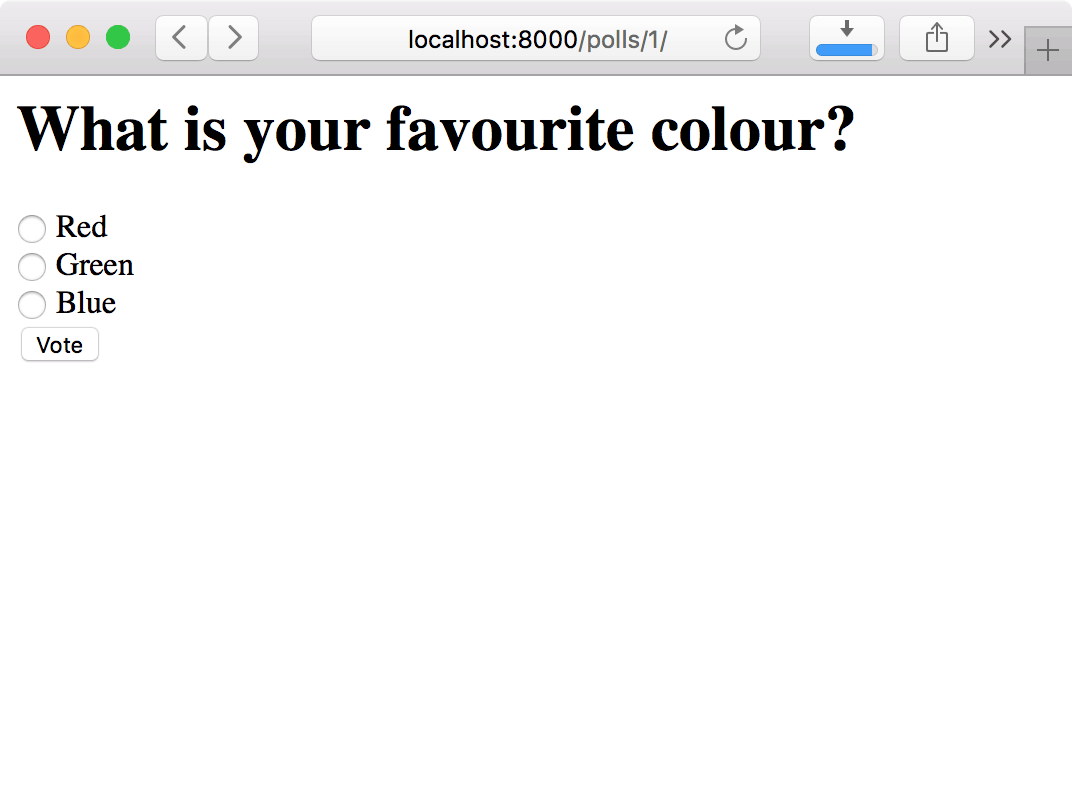
\includegraphics[width=0.95\paperwidth,center]{polls3.png}
\end{frame}
\endgroup

\begin{frame}{Getting it running}

\sizefont{3}

\begin{enumerate}
\item Install Python 3
\item \texttt{git clone https://github.com/andrewdotn/django-react.git}
\item \texttt{cd django-react}
\item \texttt{pip3 install --user -r requirements.txt}
\item \texttt{cd polls\_tutorial}
\item \texttt{./manage.py migrate}
\item \texttt{./manage.py createsuperuser}
\item \texttt{./manage.py runserver}
\end{enumerate}
\end{frame}

\section{2. JSON APIs with Django REST framework}

\begin{frame}{}
\tableofcontents[currentsection]
\end{frame}

\begin{frame}{Requirements for interactivity}

Browser needs to retrieve updated state \only<4>{GET} \\[1em]
\pause
Browser needs to update state \only<4>{POST} \\[1em]
\pause
Standard way of doing this: \\
JSON REST APIs
\pause

\end{frame}

\begin{frame}{Commits}
\begin{itemize}
\item \href{https://github.com/andrewdotn/django-react/commit/bef198f2332ab6ef492652f96aa1c46bb3a4503a}{\structure{Add serializer and view to show questions}}
\only<1>{\texttt{\\ \sizefont{2} curl http://localhost:8000/polls/api/questions/}}
\pause
\item \href{https://github.com/andrewdotn/django-react/commit/727df519b9163ed73354f878a68e21d15c9bf598}{\structure{Wire rest\_framework router to URLs}}
\\ See next slide
\end{itemize}

\end{frame}

\begingroup
\setbeamercolor{background canvas}{bg=gray}
\begin{frame}[plain]
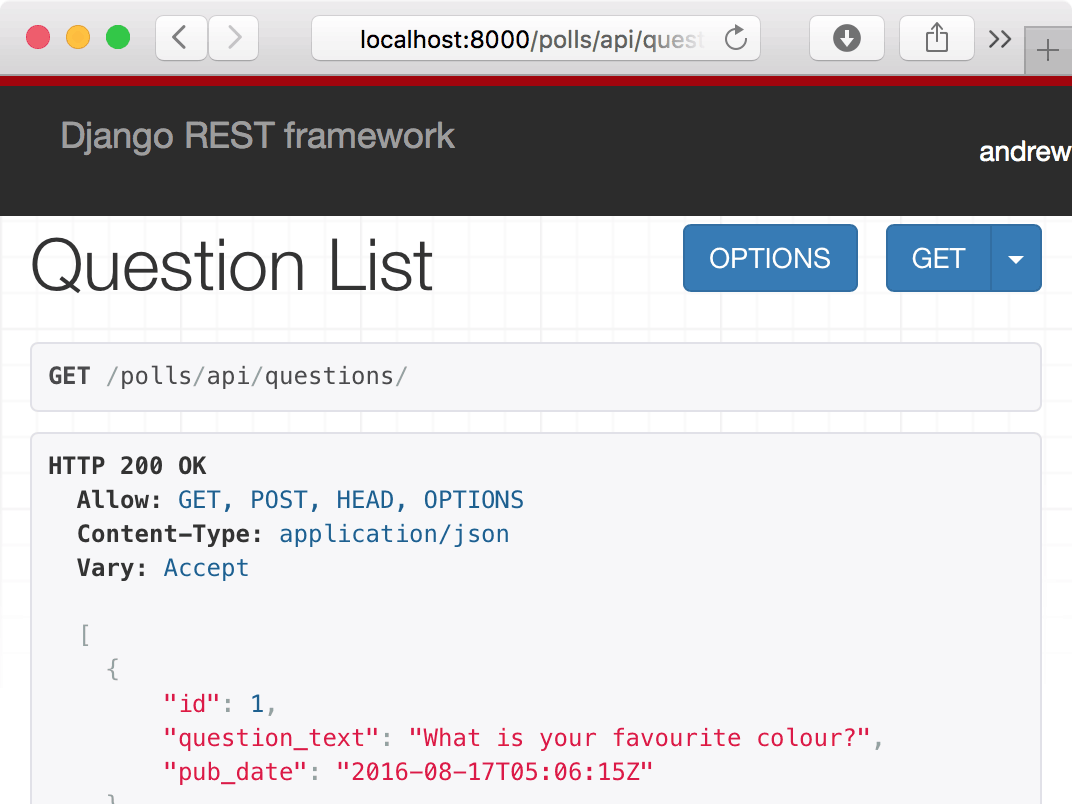
\includegraphics[width=0.95\paperwidth,center]{rest1.png}
\end{frame}
\endgroup

\begin{frame}[fragile]{Commits}
\begin{itemize}
\item \href{https://github.com/andrewdotn/django-react/commit/bef198f2332ab6ef492652f96aa1c46bb3a4503a}{\structure{Add serializer and view to show questions}}
\item \href{https://github.com/andrewdotn/django-react/commit/727df519b9163ed73354f878a68e21d15c9bf598}{\structure{Wire rest\_framework router to URLs}}
\item \href{https://github.com/andrewdotn/django-react/commit/5d9b19184e444f2d38d2ccec9c53b9d9b431b9a1}{\structure{Expose full model to API}}
\only<1>{\\ Hack to workaround namespace issues}
\pause
\item \href{https://github.com/andrewdotn/django-react/commit/89ce5e01fb8f74ffbcd53c5fce467e0c667af416}{\structure{Add increment verb}}
\end{itemize}
\sizefont{1}
\begin{verbatim}
$ curl -X POST http://localhost:8000/polls/api/choices/2/increment/; echo
{"choice_text":"0","votes":26,"question":"http://localhost:8000/polls/api/questions/2/","url":"http://localhost:8000/polls/api/choices/2/"}
$ curl -X POST http://localhost:8000/polls/api/choices/2/increment/; echo
{"choice_text":"0","votes":27,"question":"http://localhost:8000/polls/api/questions/2/","url":"http://localhost:8000/polls/api/choices/2/"}
$ curl -X POST http://localhost:8000/polls/api/choices/2/increment/; echo
{"choice_text":"0","votes":28,"question":"http://localhost:8000/polls/api/questions/2/","url":"http://localhost:8000/polls/api/choices/2/"}
\end{verbatim}
\end{frame}

\begin{frame}{Commits}
\begin{itemize}
\item \href{https://github.com/andrewdotn/django-react/commit/bef198f2332ab6ef492652f96aa1c46bb3a4503a}{\structure{Add serializer and view to show questions}}
\item \href{https://github.com/andrewdotn/django-react/commit/727df519b9163ed73354f878a68e21d15c9bf598}{\structure{Wire rest\_framework router to URLs}}
\item \href{https://github.com/andrewdotn/django-react/commit/5d9b19184e444f2d38d2ccec9c53b9d9b431b9a1}{\structure{Expose full model to API}}
\item \href{https://github.com/andrewdotn/django-react/commit/89ce5e01fb8f74ffbcd53c5fce467e0c667af416}{\structure{Add increment verb}}
\end{itemize}
Your turn!
\end{frame}

\section{3. Interactivity with React.js}

\begin{frame}{}
\tableofcontents[currentsection]
\end{frame}

\begin{frame}{React.js}

The new standard for JS frontend work \\[1em] \pause

Rules:
\pause
\begin{itemize}
\item Components render HTML as a function of properties and state
\pause
\item Properties can only be changed by parent components
\pause
\item Visual updates only happen when properties or state change in a way
that affects the output of the render function
\end{itemize}

\end{frame}

\begin{frame}{Commits}
\begin{itemize}
\item \href{https://github.com/andrewdotn/django-react/commit/6dc5466a174ec3265c0590c33c2328316eb4c34d}{\structure{React hello world}}
\pause
\only<2>{ \\ Note that including the initial JSON in the response saves
round-trips aka progress spinner time }
\pause
\item \href{https://github.com/andrewdotn/django-react/commit/4ba8f0ad16afc44233c88e0b1bc62f2ca9674aa9}{\structure{Format questions}}
\pause
\item \href{https://github.com/andrewdotn/django-react/commit/bec0411c648b2668f7977a75a461e11534073e0e}{\structure{Render vote counts in tables}}
\pause
\only<5>{\\ \texttt{key} allows for insertions, deletions, and reordering}
\pause
\item \href{https://github.com/andrewdotn/django-react/commit/243f7d4e5f7bde54fdeb147198cf21ed105560c7}{\structure{Add polling for data updates}}
\pause
\only<7>{\\ excellent separation of concerns}
\pause
\item \href{https://github.com/andrewdotn/django-react/commit/3e93a9cf1a2c8e772abf3a7913267cfeed6649de}{\structure{Implement increment call with react}}
\pause
\only<9>{\\ normally you’d use callbacks instead of
\texttt{componentWillReceiveProps}}
\end{itemize}
\end{frame}

\begin{frame}{Demo}
\end{frame}

\section{Conclusion}

\begin{frame}{}
\tableofcontents[currentsection]
\end{frame}

\begin{frame}{Conclusions}
\begin{itemize}
\item Exposing an API for your existing models is pretty straightforward
\pause
\item React.js is an in-browser template layer that lets you add live
updates without changing rendering code
\end{itemize}
\end{frame}

\begin{frame}{Future work}
\begin{itemize}
\item \alert<5>{Replicate}
\pause
\item Pause/faster/slower controls on polling
\pause
\item Permissions
\pause
\item Pre-compile JSX
\pause
\item WebSockets
\end{itemize}
\end{frame}

\end{document}
